\documentclass[12pt,a4paper,twoside]{article}

\usepackage{amsmath}
\usepackage{amsfonts}
\usepackage{amssymb}
\usepackage{graphicx}
\usepackage{caption}
\usepackage{fancyhdr}
\usepackage{lastpage}
\usepackage{wrapfig}
\usepackage{color}
\usepackage{fancybox}
\usepackage[T1]{fontenc}
% \usepackage{hangcaption}
\usepackage{listings}
\usepackage[utf8]{inputenc}
\usepackage[francais]{babel}
\usepackage{parskip}
\usepackage{float}
\usepackage{enumitem}

\newcommand{\hsp}{\hspace{20pt}}
\newcommand{\HRule}{\rule{\linewidth}{0.5mm}}

\usepackage[a4paper,left=2cm,right=2cm,top=2cm,bottom=2cm]{geometry}

\geometry{
margin=2.5cm,
includeheadfoot,
}

%\usepackage{libertine}
\author{Antoine Roche}
\title{Rapport de Stage}

\setlength{\parindent}{2em}
\begin{document}

    \begin{titlepage}                                    %%% PAGE DE GARDE %%%
        \begin{sffamily}
            \begin{center}

                % Upper part of the page. The '~' is needed because \\
                % only works if a paragraph has started.

                %% Les deux images cote à cote
                \begin{figure}[h]
                    \begin{minipage}[c]{.46\linewidth}
                        \centering
                        
\includegraphics[scale=0.2]{ressources/images/logos/Logo_Reims_University.png}
                        %\caption*{Cea}
                    \end{minipage}
                    \hfill%
                    \begin{minipage}[c]{.46\linewidth}
                        \centering
                        
\includegraphics[scale=0.1]{ressources/images/logos/logo_cea.png}
                    \end{minipage}
                \end{figure}
                \vspace{2cm}
                \textsc{\LARGE Université de Reims Champagne-Ardenne}\\[2cm]
                \textsc{\Large Rapport de stage Master 1}\\[1.5cm]
                % Title
                \HRule \\[1cm]
                { \Large \bfseries Etude et évaluation de la structure de donnée SVDAG et ses variantes pour le RayTracing en visualisation scientifique \\[0.4cm] }
                \HRule \\[2cm]

                % Author and supervisor

                \begin{minipage}{0.8\textwidth}
                    \begin{flushleft}
                        \Large Auteur: \textsc{Antoine Roche}\\
                        Tuteur de stage: \textsc{Jérôme Dubois}\\
                        Tuteur enseignant : \textsc{Mickael Krajecki}\\
                    \end{flushleft}
                \end{minipage}

                \vfill
                \Large 08/04/2019 — 30/08/2019 \\[1cm]
                \Huge {CEA, DAM, DIF, F-91297, Arpajon, France}
                % Bottom of the page

            \end{center}
        \end{sffamily}
    \end{titlepage}

\newpage
    \section*{Remerciements}

    Je tiens à remercier Jérôme Dubois et Jacques-Bernard Lekien pour leur aide précieuse, ainsi que l'occasion d'avoir participé
    à la VISU2019 pour présenter mon travail et prendre connaissance de celui d'autres chercheurs dans le milieu de la visualisation.
    Je remercie également Michael Krajecki pour m'avoir donné l'opportunité de travailler au sein du CEA.


    \newpage

    \renewcommand{\contentsname}{Sommaire}

    \tableofcontents


    \newpage

    \lstset{numbers=left, tabsize=3, frame=single, numberstyle=\ttfamily,
    basicstyle=\footnotesize}
    \thispagestyle{empty}

    \section{Introduction}                          %%% INTRODUCTION %%%



    Le CEA, acteur majeur en matière de recherche et d’innovation, est considéré comme étant un expert du Calcul Haute
    Performance. Dans ce contexte, les équipes spécialisées en visualisation scientifique sont reconnues pour
    leur expertise en visualisation parallèle sur supercalculateur. Elles participent activement au développement de la
    bibliothèque open-source VTK, qui fournit un pipeline complet de visualisation associant différents types de données
    et d’algorithmes.

    Pour répondre aux besoins de codes de simulation, le CEA a développé depuis quelques années des
    structures de données et des filtres VTK dédiés à la visualisation et la manipulation de maillages AMR. D’autres
    structures hiérarchiques utilisées dans le cadre de l’industrie cinématographique ou du jeux-vidéo permettent un rendu
    réaliste de type ray-tracing en temps réel en faisant appel à la programmation sur carte graphique (CUDA).

    Ces structures
    sont basées sur les Sparse Voxel Octrees (SVO), une représentation d’une scène voxelisée de type octree optimisée.
    Des techniques de compressions offrent par la suite des gains substantiels en tenant compte des motifs similaires :
    les Sparse Voxel Directed Acyclic Graph (SVDAG) ou encore les Symmetric SVDAG (SSVDAG).
    L’objectif du stage est de permettre l’évaluation de ces structures hiérarchiques pour la visualisation scientifique.

    \newpage

    \section{Présentation CEA}                              %%% PRESENTATION CEA %%%

    Acteur majeur de la recherche, du développement et de l'innovation, le Commissariat à l’énergie atomique et aux énergies alternatives intervient dans quatre domaines :

    \begin{itemize}[label=\textbullet]
        \item    La défense et la sécurité. ;
        \item    Les énergies bas carbone (nucléaires et renouvelables). ;
        \item    La recherche technologique pour l’industrie. ;
        \item    La recherche fondamentale (sciences de la matière et sciences de la vie).
    \end{itemize}

    S’appuyant sur une capacité d’expertise reconnue, le CEA participe à la mise en place de projets de collaboration
    avec de nombreux partenaires académiques et industriels. Le CEA est implanté sur 9 centres répartis dans toute la
    France. Il développe de nombreux partenariats avec les autres organismes de recherche, les collectivités locales
    et les universités. A ce titre, le CEA est partie prenante des alliances nationales coordonnant la recherche
    française dans les domaines de l’énergie (ANCRE), des sciences de la vie et de la santé (AVIESAN), des sciences
    et technologies du numérique (ALLISTENE), des sciences de l’environnement (AlIEnvi) et des sciences humaines et
    sociales (ATHENA).

    Reconnu comme un expert dans ses domaines de compétence, le CEA est pleinement inséré dans l'espace européen de
    la recherche et exerce une présence croissante au niveau international. Le CEA compte 15 942 techniciens,
    ingénieurs, chercheurs et collaborateurs pour un budget de 5 milliards d'euros (chiffres publiés fin 2017).

    \begin{figure}[b]
        \centering
        \makebox[\textwidth]{
        \raisebox{-80pt}[0pt][70pt]{
        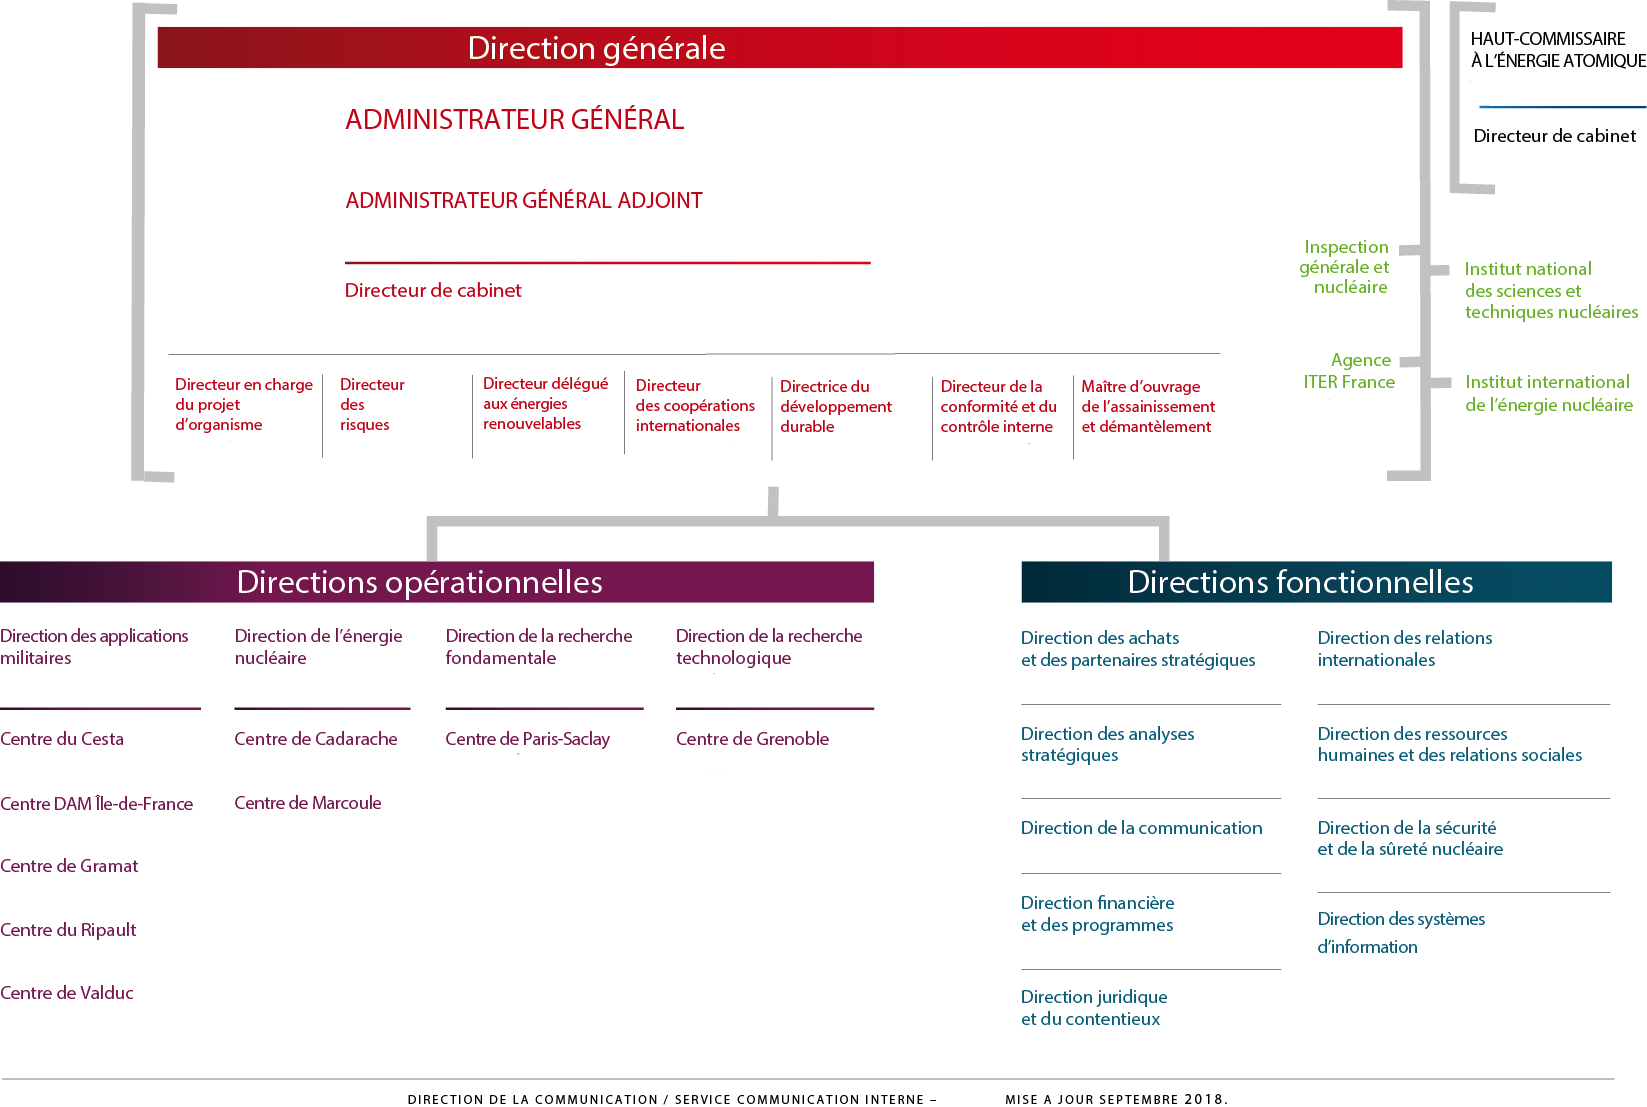
\includegraphics[width=0.8\textwidth]{ressources/diagrammes/organigramme_cea.png}
        }
        }
    \end{figure}

    \newpage

    \section*{La direction des applications militaires}

    \subsection*{Une direction au service de la dissuasion}
    La Direction des applications militaires (DAM) du CEA, a pour mission
    de concevoir, fabriquer, maintenir en condition opérationnelle, puis démanteler
    les têtes nucléaires qui équipent les forces nucléaires aéroportée et océanique
    françaises.

    La DAM est chargée de la conception et de la réalisation des réacteurs et de
    c\oe urs nucléaires équipant les bâtiments de la Marine nationale, sous-marins
    et porte-avions. Elle apporte son soutien à la Marine nationale pour le suivi en
    service et le maintien en condition opérationnelle de ces réacteurs.

    La DAM est également responsable de l'approvisionnement des matières nucléaires
    straté\-giques pour les besoins de la dissuasion.

    Dans un monde en profonde mutation, la DAM contribue aussi à la sécurité
    nationale et
    \begin{wrapfigure}[12]{r}{10cm}
        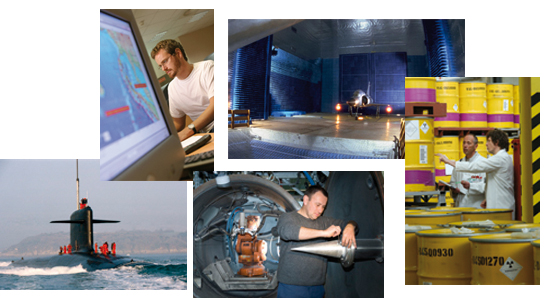
\includegraphics[width=10cm]{ressources/images/dam/5_thumbnails.jpg}
    \end{wrapfigure}
    internationale à travers l'appui technique qu'elle apporte aux autorités, pour
    les questions de lutte contre la prolifération nucléaire et le terrorisme et de
    désarmement.

    Depuis le transfert du centre de Gramat en 2010 de la Direction générale de
    l'armement au CEA, la DAM apporte son expertise à la Défense dans le domaine de
    l'armement conventionnel.

    \subsection*{Une direction ouverte à la recherche}
    Le partage national et international des connaissances (lorsqu'il est possible),
    la confrontation à l'évaluation scientifique extérieure, l'intégration à des
    réseaux de compétences constituent des gages de crédibilité scientifique.

    Les équipes de la DAM réalisent chaque année environ 2000 publications et
    communications scientifiques. Cette ouverture de la DAM passe également par la
    mise à la disposition de la communauté des chercheurs de ses moyens
    expérimentaux et par la contribution de ses équipes à d'autres programmes de
    recherche.

    \subsection*{Une direction actrice de la politique industrielle française}
    La DAM partage très largement son activité avec l'industrie française : c'est
    ainsi que le montant des achats, auprès de celle-ci, représente plus des deux
    tiers de son budget ; le dernier tiers se répartit entre les salaires des
    personnels (un cinquième) et les taxes.

    La politique industrielle de la DAM est originale à plus d'un titre :

    \begin{itemize}[label=\textbullet]
        \item
        d'abord parce que la DAM conserve la maîtrise d'\oe uvre
        d'ensemble de la grande majorité des systèmes dont elle a la
        responsabilité : elle veille ainsi au juste équilibre entre les
        grands groupes industriels de la Défense et les PME souvent
        innovantes, en contractualisant directement avec ces dernières,
        leur permettant ainsi de recevoir la juste rémunération de leur
        production ;
        \item
        ensuite, parce que la répartition de son budget est sous-tendue
        par une répartition des travaux : la DAM conduit la recherche
        dans ses laboratoires grâce à son personnel de haut niveau
        scientifique et technologique. Une fois la définition d'un
        produit acquise, la DAM transfère la définition et les procédés
        vers les industriels qui en réalisent le développement, puis la
        production.
    \end{itemize}

    La DAM a également pour objectif que ses centres participent à la vie économique
    locale par leur implication dans les pôles de compétitivité. Hors de son propre
    champ d'utilisation, elle valorise ses recherches par le transfert de
    technologies vers l'industrie et le dépôt de nombreux brevets.

    \subsection*{Le format}
    La DAM comprend cinq centres aux missions homogènes, dont les activités se
    répartissent entre la recherche de base, le développement et la fabrication :
    \begin{figure}[!ht]
        \begin{minipage}{0.6\linewidth}
            \begin{itemize}[label=\textbullet]
                \item
                {\bf DAM Ile-de-France (DIF)}, à Bruyères-le-Châtel, où sont
                menés les travaux de physique des armes, les activités de
                simulation numérique et de lutte contre la prolifération
                nucléaire ; DIF est aussi le centre responsable de l'ingénierie
                à la DAM ; enfin, au centre DIF est rattachée l'INBS-Propulsion
                Nucléaire du centre CEA/Cadarache, en région Provence Alpes-Côte
                d'Azur, où sont implantées les installations d'essais à terre et
                une partie des fabrications de la propulsion nucléaire ;
            \end{itemize}
        \end{minipage}
        \begin{minipage}{0.4\linewidth}
            \centering
            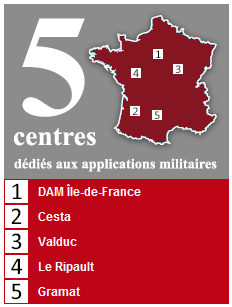
\includegraphics[width=0.7\textwidth]{ressources/images/dam/5_centres.png}
        \end{minipage}
    \end{figure}

    \begin{itemize}[label=\textbullet]
        \item
        {\bf Le Cesta}, en Aquitaine, consacré à l'architecture des armes, aux
        tests de tenue à l'environnement. Il met en oeuvre le Laser Mégajoule,
        équipement majeur de la Simulation ;
        \item
        {\bf Valduc}, en Bourgogne, dédié aux matériaux nucléaires et à
        l'installation expérimentale Epure du programme Simulation ;
        \item
        {\bf Le Ripault}, en région Centre, dédié aux matériaux non nucléaires
        (explosifs chimiques\textellipsis) ;
        \item
        {\bf Gramat}, (ex-DGA) en Midi-Pyrénées, qui conduit au profit de la
        Défense des activités en vulnérabilité des systèmes et efficacité des
        armements. ;
    \end{itemize}



    \newpage
    \section*{Le centre DAM Ile-de-France}
    \begin{figure}[H]
        \centering
        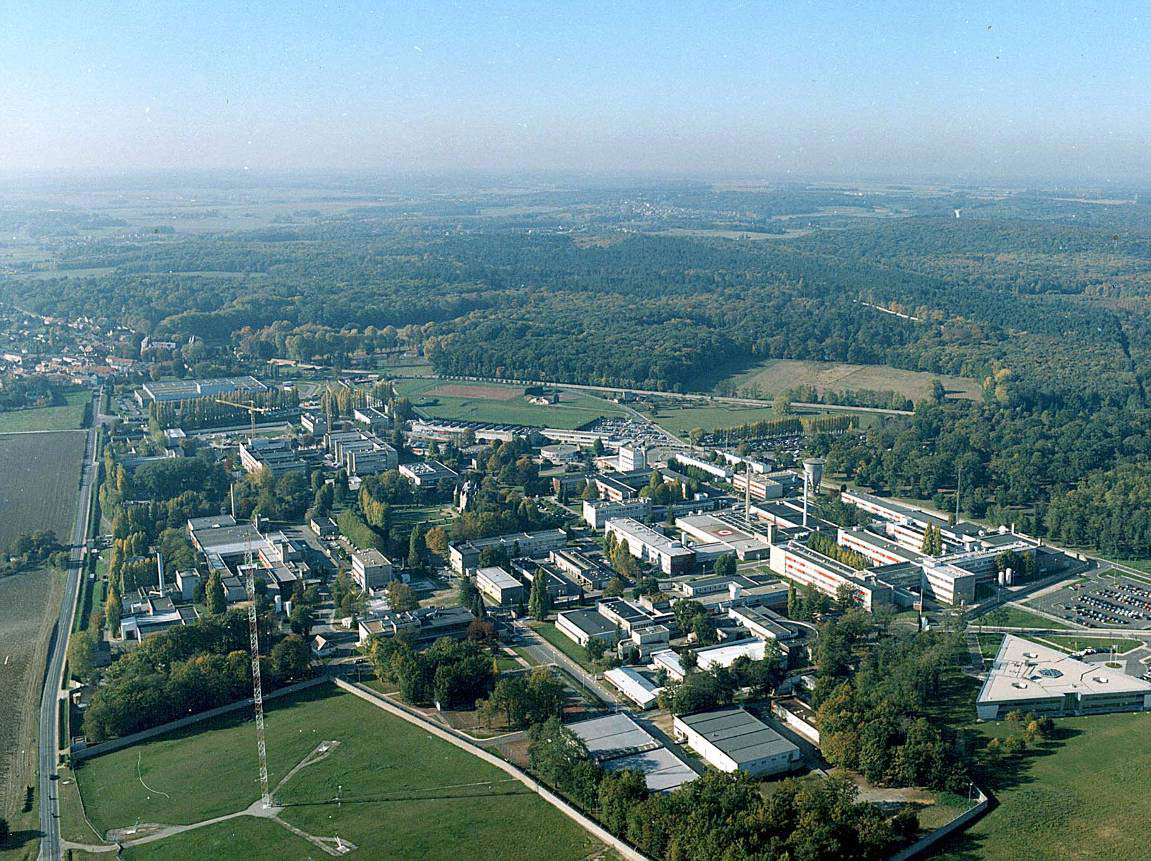
\includegraphics[scale=0.4]{ressources/images/dam/vue_aerienne.png}
        \caption*{Centre DAM Île-de-France}
    \end{figure}

    Le CEA/DAM - Île de France (DIF) est l'une des directions opérationnelles de la DAM. Le site de la DIF compte
    environ 2000 salariés CEA et accueille quotidiennement environ 600 salariés d'entreprises extérieures. Il est
    situé à Bruyères-le-Châtel à environ 40 km au sud de Paris, dans l'Essonne.

    Les missions de la DIF comprennent :

    \begin{itemize}[label=\textbullet]
        \item
        La conception et garantie des armes nucléaires, grâce au programme Simulation. L'enjeu consiste à reproduire par le calcul les différentes phases du fonctionnement d'une arme nucléaire et à confronter ces résultats aux mesures des tirs nucléaires passés et aux résultats expérimentaux obtenus sur les installations actuelles (machine radiographique, lasers de puissance, accélérateurs de particules). ;
        \item
        La lutte contre la prolifération et le terrorisme, en contribuant notamment au programme de garantie du Traité de Non-Prolifération et en assurant l'expertise technique française pour la mise en œuvre du Traité d'Interdiction Complète des Essais Nucléaires (TICE).
        \item
        L'expertise scientifique et technique, dans le cadre de la construction et du démantèlement d'ouvrages complexes ainsi que pour la surveillance de l'environnement et les sciences de la terre.
        \item
        L'alerte des autorités, mission opérationnelle assurée 24h sur 24, 365 jours par an, en cas d'essai nucléaire, de séisme en France ou à l'étranger, et de tsunami dans la zone Euro-méditerranéenne. La DIF fournit aux autorités les analyses et synthèses techniques associées.

    \end{itemize}

    Depuis 2003, le centre DAM-Île-de-France héberge le complexe de calcul scientifique du CEA, qui regroupe l’ensemble des supercalculateurs du CEA, et qui comprend à ce jour :

    \begin{itemize}[label=\textbullet]
        \item
        Le supercalculateur Tera1000-1 pour les besoins du programme Simulation du CEA/DAM, mis en service en 2016, dispose d’une puissance de calcul de 2,5 petaflops, c’est à dire capable d’effectuer 2,5 millions de milliards d’opérations par seconde. Il est complété en 2018 par Tera1000-2, autre composante du projet Tera1000, qui préfigure les architectures et technologies du futur supercalculateur qui sera installé à l’horizon 2020.Sa puissance de calcul est de 12,5 petaflops.

        \begin{figure}[H]
            \centering
            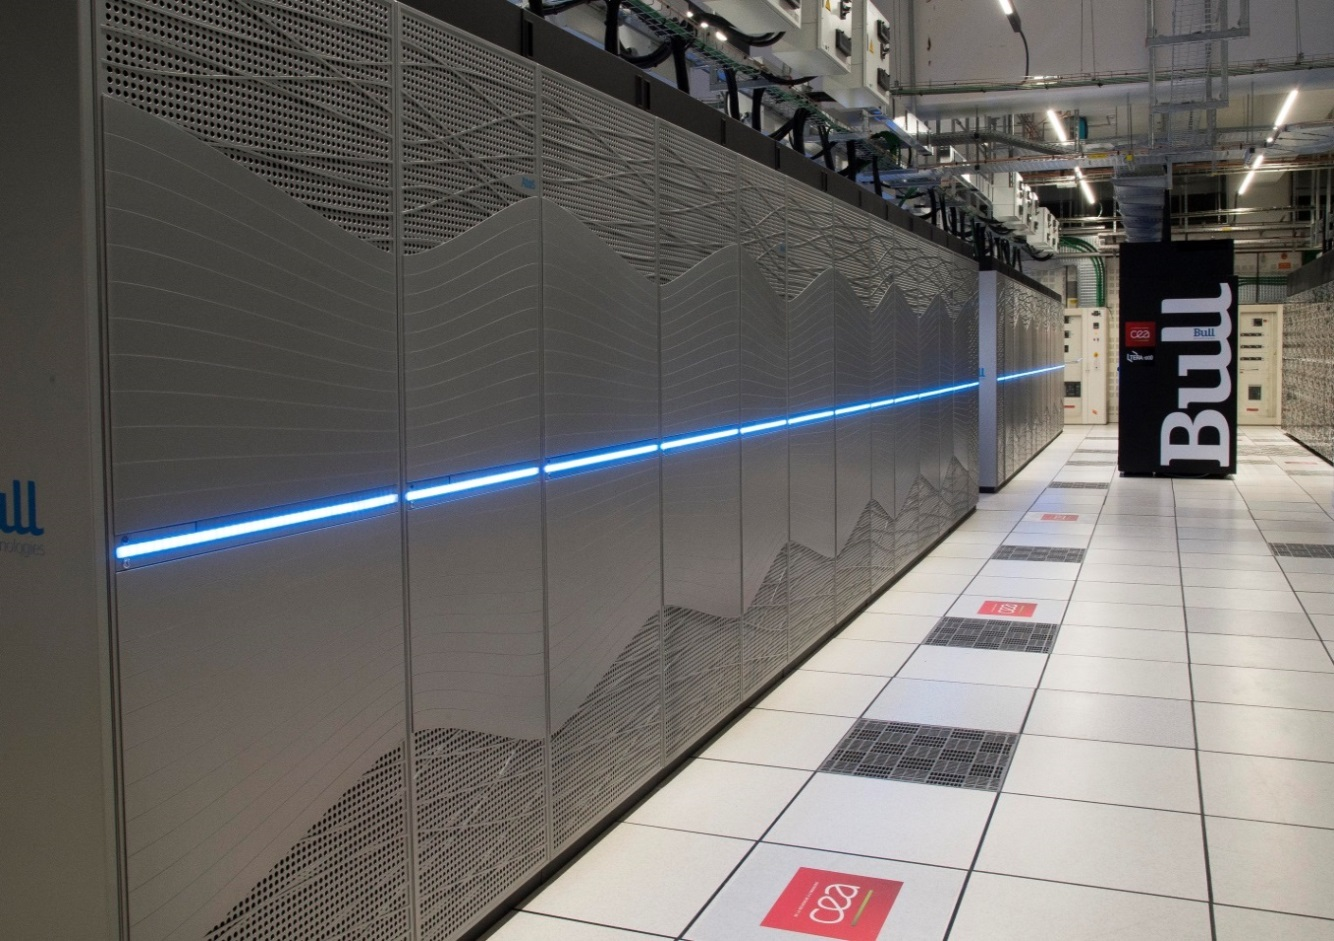
\includegraphics[scale=1]{ressources/images/dam/tera1000.jpg}
        \end{figure}

        \item
        Le supercalculateur Cobalt du Centre de Calcul pour la Recherche et la Technologie (CCRT), ouvert à la communauté civile de la recherche et de l’industrie, pour une puissance globale de 1,5 petaflops.
        \begin{figure}[H]
            \centering
            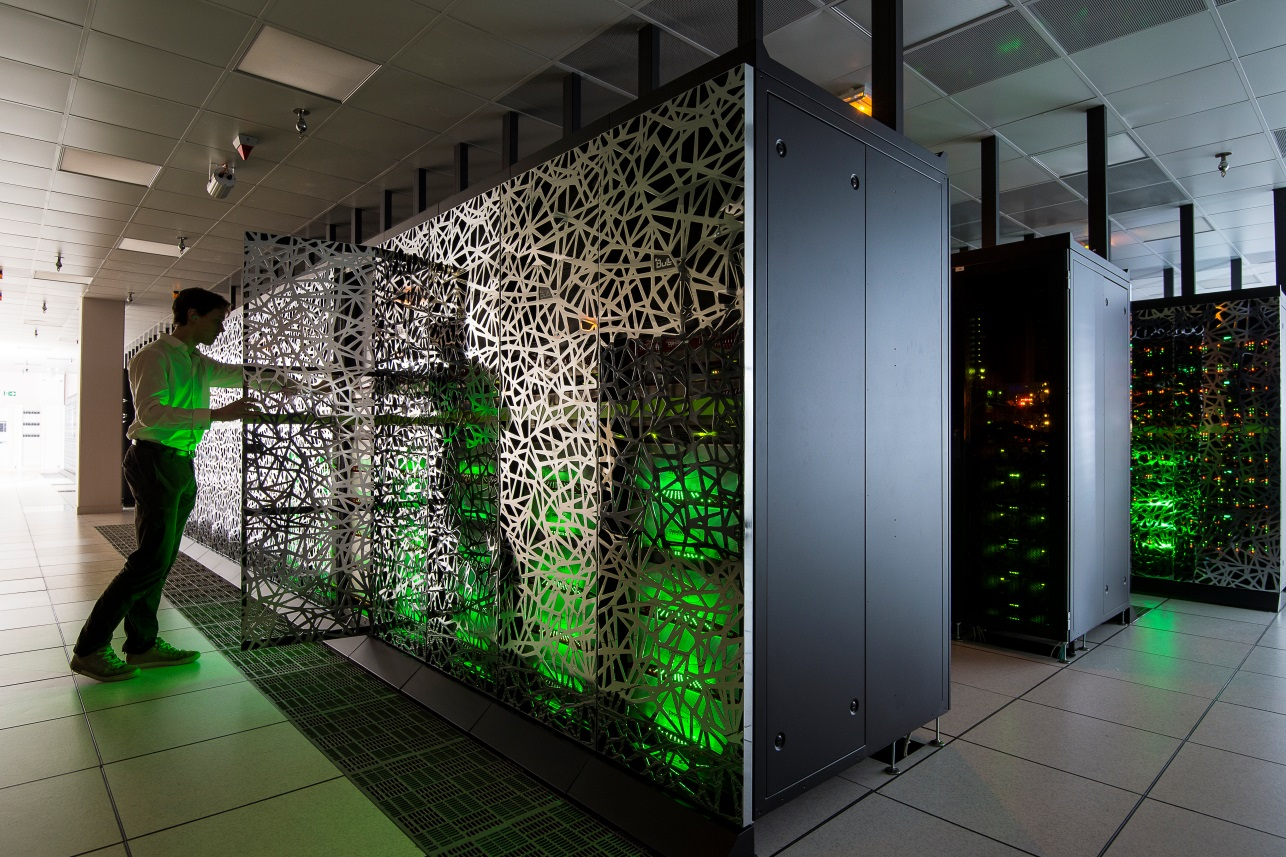
\includegraphics[scale=1]{ressources/images/dam/cobalt.jpg}
        \end{figure}

        \item
        Le supercalculateur IRENE, d’une puissance de 9 petaflops, deuxième élément d’un réseau de supercalculateurs de classe petaflopique destiné aux chercheurs de la communauté scientifique européenne. Ce supercalculateur est hébergé au TGCC (Très Grand Centre de Calcul) et exploité par les équipes du CEA, qui apporte ainsi sa contribution à la participation de la France au projet PRACE (Partnership for Advanced Computing in Europe)

    \end{itemize}



    \newpage


    \newpage
    \section{Contexte du stage}                 %%% PRESENTATION STAGE %%%

    Etant en collaboration directe avec l'équipe de visualisation du CEA, le but de mon stage est d'appliquer
    des technologies du jeu vidéo sur de la visualisation scientifique. Plus précisement, mon objectif est de convertir
    une structure VTK-AMR, technologie nouvelle dans le domaine de la visualisation scientifique permettant de réduire
    le volume et le temps de rendu de données de simulations massives, vers une structure SVDAG, appliquée notamment pour
    du raytracing sur des décors de jeux vidéo, qui permet de compresser un octree sans perte de données.

    Ces deux technologies sont très puissantes dans leur domaine respectif. Elle peuvent permettre le rendu de scènes
    très massives, initialement visualisable uniquement sur supercalculateur, sur des ordinateurs portables bon marché.

    Afin de mener le projet jusqu'à son terme, je dois tout d'abord étudier et comprendre la théorie et l'implémentation des structures
    SVO/SVDAG/SSVDAG pour en évaluer les performances de rendu raytracing sur des modèles connus. Pour cela, je suis en contact
    avec les équipes de recherche suédoise à la base du SVDAG, avec lesquels je pourrai donc collaborer.

    D'un autre côté, je dois comprendre et maitriser la construction de structure AMR via VTK. Je dois notamment
    savoir construire un AMR à partir d'un SVO et avoir un résultat visuel identique au SVO en entrée.

    Une fois la phase de recherche terminée, un premier convertisseur VTK-AMR vers SVDAG/SSVDAG sera à
    implémenter. Des tests de performances s'en suivront afin de les comparer avec celles des autres structures.

    Pour finir, le travail se poursuivra par l'application de rendu réaliste de type lancé de rayons à base de SVDAG sur
    des données issues de VTK-AMR. Plusieurs développements seront possibles en vue de prendre en compte la notion de variables ou de
    compresser encore plus les informations dans le cadre de rendu de films interactifs. Les développements effectués seront
    évalués aussi bien sur GPU (CUDA) que sur les nombreux accélérateurs et processeurs disponibles au CEA.

    \newpage
    \section{Etudes menées}     %%% ETUDES MENEES %%%

    Dans le cadre du stage, des études préliminaires étaient nécessaires afin de comprendre les structures de données que
    j'allais manipuler.

    \subsection{Sparse Voxel Octree}

    Le Sparse Voxel Octree (SVO) est la structure de base à connaître afin de comprendre les autres.
    Pour cela, je me suis basé sur la thèse de Viktor Kämpe sur le SVDAG ainsi que le papier de recherche de NVIDIA
    Research sur le ESVO, car ils introduisent le SVO de sorte à comprendre le reste.

    Le SVO est une représentation de données en arbre. Sa structure permet d'accéder à une information rapidement.
    Il est construit à partir d'une scène 3D non structurée, qui est ensuite découpée en grille dont les cases contenant un élément sont à leur tour découpées jusqu'à atteindre le niveau défini.
    Chaque feuille du dernier niveau devient alors un voxel.

    \begin{figure}[H]
        \centering{
        \resizebox{70mm}{!}{\input{ressources/inkscape/SVO1.pdf_tex} \space \space \input{ressources/inkscape/SVO2.pdf_tex}}
        \caption{Découpage d'une scène 2D avec 3 niveaux et représentation des "voxels" obtenus}
        \label{fig:svo1}
        }
    \end{figure}


    \begin{figure}[H]
        \centering{
        \resizebox{130mm}{!}{\input{ressources/inkscape/SVO3.pdf_tex}}
        \caption{Représentation de l'arbre construit}
        \label{fig:svo3}
        }
    \end{figure}

    \subsection{Sparse Voxel Directed Acyclic Graph}

    Pour le Sparse Voxel Directed Acyclic Graph (SVDAG), j'ai de nouveau utilisé la thèse de Victor Kämpe ainsi que le papier
    "High Resolution Sparse Voxel Dags" écrit par Victor Kämpe, Erik Sintorn et Ulf Assarsson. J'ai également étudié le
    programme qu'ils ont partagé, muni d'un jeu de donnée en exemple.

    Le SVDAG est un arbre de voxel compressé. Il peut être construit à partir d'un SVO.
    Sa particularité est qu'un noeud peut être pointé par plusieurs parents, évitant ainsi de stocker plusieurs noeuds s'ils sont identiques.
    Il est également acyclic, nous pouvons descendre dans l'arbre mais pas remonter. Cela offre un gain de stockage supplémentaire en ne spécifiant pas les parents des noeuds.
    Tout cela permet de faire tenir en mémoire des structures trop volumineuses à la base et de rendre les accès mémoires plus rapides.

    \begin{figure}[H]
        \centering{
        \resizebox{80mm}{!}{\input{ressources/inkscape/svdag1.pdf_tex}}
        \caption{Représentation d'un arbre de données}
        \label{fig:svdag1}
        }
    \end{figure}

    \begin{figure}[H]
        \centering{
        \resizebox{35mm}{!}{\input{ressources/inkscape/svdag2.pdf_tex}}
        \caption{Représentation de l'arbre après compression via SVDAG}
        \label{fig:svdag2}
        }
    \end{figure}
    \newpage
    \subsection{Adaptive Mesh Refinement}

    Prendre connaissance de l'Adaptive Mesh Refinement (AMR) fut plus basé sur des explications venant de
    Jérôme Dubois et Jacques-Bernard Lekien qui m'ont également fourni des programmes exemples. Je me suis tout de même
    appuyé sur une présentation de Massimiliano Guarrasi, introduisant l'AMR et les outils associés.

    L'AMR est un arbre semblable au SVO, à la grande différence que les voxels peuvent se situer à des niveaux différents dans l'arbre.
    Ceci implique qu'une scène peut contenir des voxels plus grossiers que d'autres si un affinage n'est pas nécessaire.
    En contrepartie, des zones peuvent être très détaillées sans allourdir la mémoire de façon excessive. \\
    De plus, il est aisé de diminuer le niveau maximal des voxels pour obtenir une scène moins détaillée
    mais beaucoup plus fluide (voire en temps réel) afin de configurer rapidement les différents paramètres pour le rendu final.

    \begin{figure}[H]
        \centering{
        \resizebox{100mm}{!}{\input{ressources/inkscape/amr_grille1.pdf_tex} \space \space \input{ressources/inkscape/amr_arbre1.pdf_tex}}
        \caption{Grille de type AMR de niveau 3 avec son arbre associé}
        \label{fig:amr1}
        }
    \end{figure}

    \begin{figure}[H]
        \centering{
        \resizebox{100mm}{!}{\input{ressources/inkscape/amr_grille2.pdf_tex} \space \space \input{ressources/inkscape/amr_arbre2.pdf_tex}}
        \caption{Grille de type AMR de niveau 2 avec son arbre associé}
        \label{fig:amr2}
        }
    \end{figure}

\section{Travail réalisé}

    \subsection{Prises de connaissances}

    La première semaine du stage fut dédiée à la connaissance et à la compréhension des structures de données citées plus haut.
    Pour cela, j'ai lu plusieurs papiers de recherche, de manière plus ou moins appronfondie.

    \subsection{Installation de l'environnement}

    Plusieurs semaines ont ensuite été dédiées à l'installation de l'environnement nécessaire.
    N'ayant pas les droits d'administrateur, j'ai installé Spack en tant que gestionnaire de paquets.\\
    J'ai ensuite installé VTK, contenant des modules pour l'AMR, et le programme SVDAG fourni, ainsi que toutes les dépendences.

    \subsection{Installation et fonctionnement du programme SVDAG}

    Contrairement à tous les autres code sources, celui du SVDAG a été fait sur Windows. J'ai donc du résoudre les problèmes
    de compatibilité, notamment causés par un paquet dépendant au système. \\
    Le programme était maintenant fonctionnel, et le fichier d'entrée donné en exemple également.
    Afin d'utiliser d'autres fichiers en entrée, j'ai du chercher et installer un constructeur de SVO. Je l'ai également
    modifié de sorte à sortir les fichiers aux bons formats, pour qu'ils soient compatibles avec le SVDAG.
    De l'autre côté, j'ai ajusté l'entrée du SVDAG. J'ai également ajouté une option permettant d'écrire le SVDAG sur
    le disque pour ne pas avoir à le construire à chaque fois que l'on veut le visualiser.


    \subsection{Analyse des performances du SVDAG}

    Avec tout en place, j'ai pu tester le programme afin de comprendre comment il se comporte selon différents
    paramètres. J'ai également analysé ses performances avec quelques jeux de données connus.

    \subsubsection{Résultats}

    \begin{figure}[H]
        \centering
        \resizebox{160mm}{!}{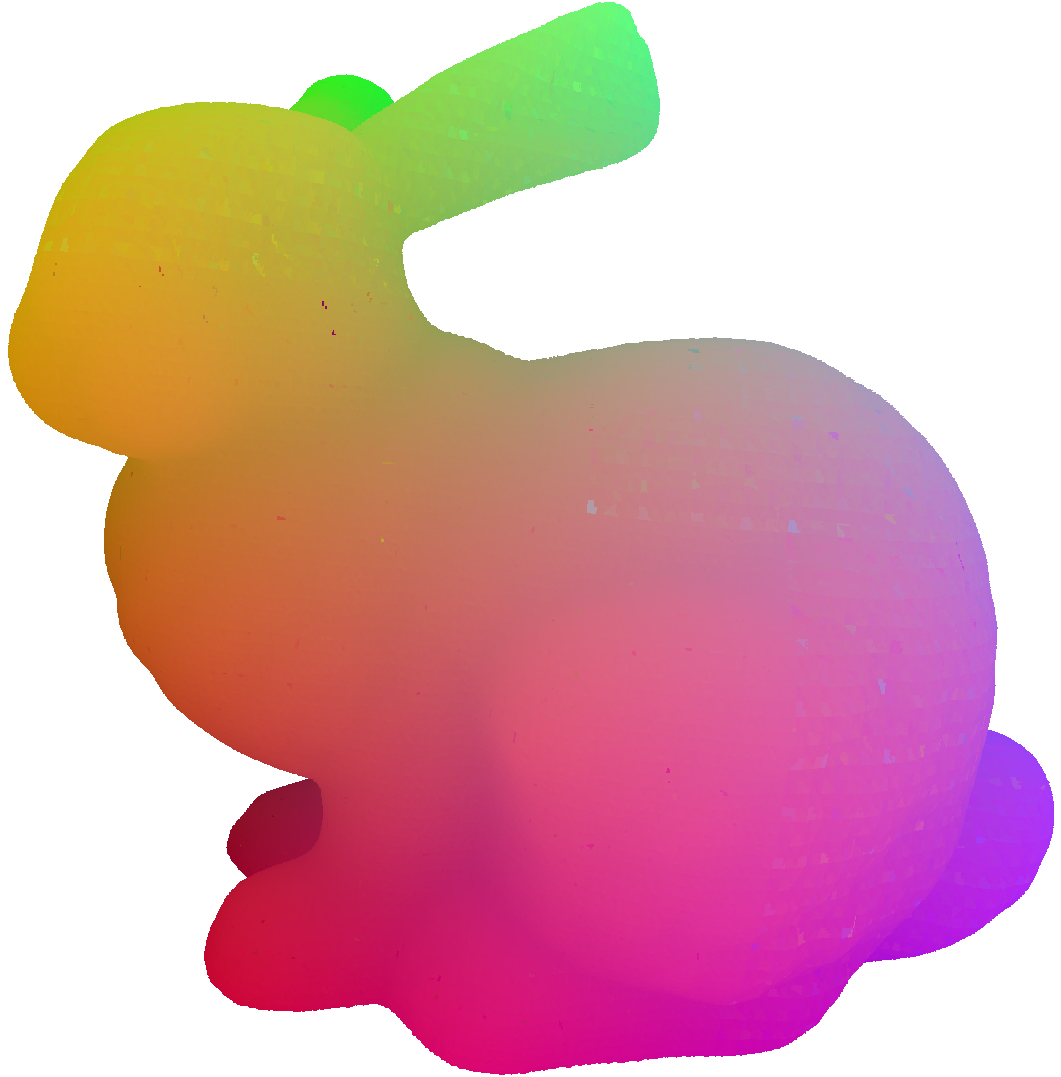
\includegraphics[width=0.2\linewidth]{ressources/images/bunny.png}
        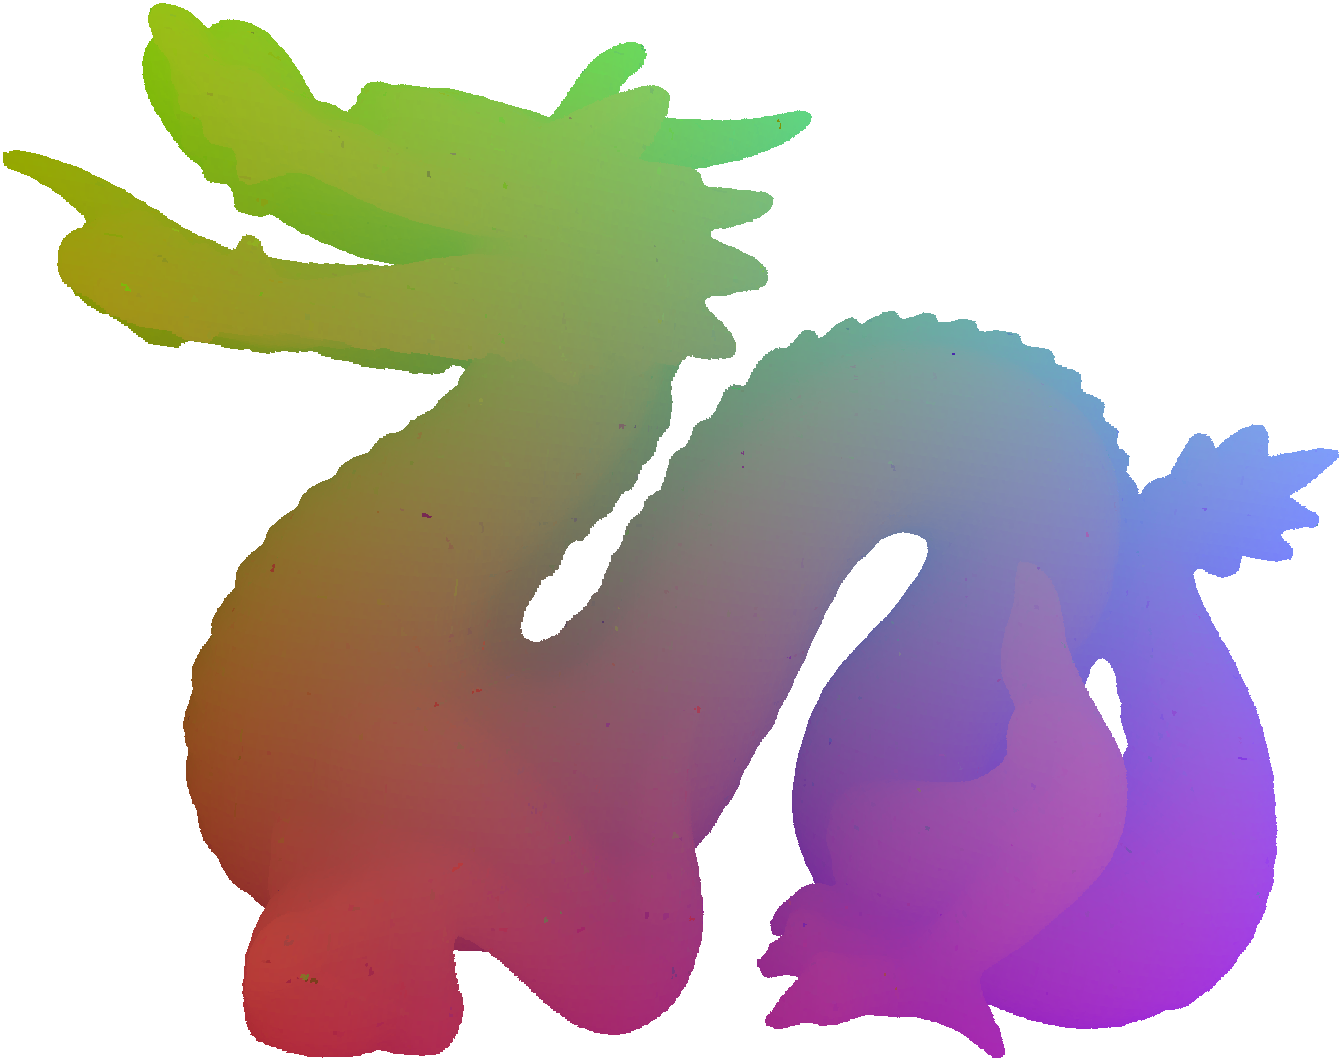
\includegraphics[width=0.2\linewidth]{ressources/images/dragon.png}
        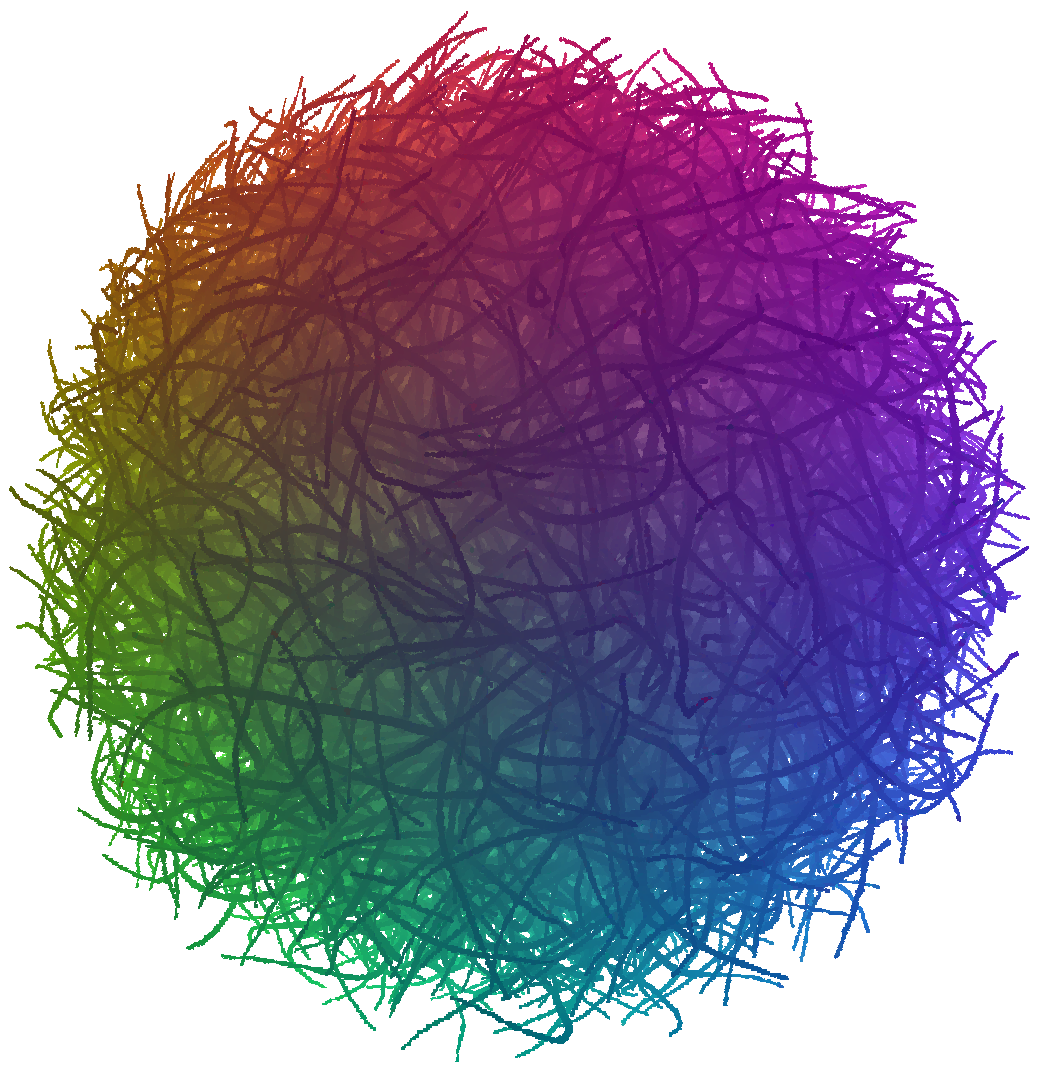
\includegraphics[width=0.2\linewidth]{ressources/images/hairball.png}
        
\includegraphics[width=0.2\linewidth]{ressources/images/lucy.png}}
        \caption{Rendu de modèles avec du raycasting sur SVDAG}
        \begin{center}
            De gauche à droite : Bunny (Stanford), Dragon (Stanford), Hairball (NVIDIA Research), Lucy (Stanford)
        \end{center}
        \label{models}
    \end{figure}




    \begin{table}[H]
        \begin{tabular}{lllll}
            \hline
            \multicolumn{1}{|l|}{}         & \multicolumn{1}{l|}{\begin{tabular}[c]{@{}l@{}}
                                                                     Nombre\\ Triangles
            \end{tabular}} & \multicolumn{1}{l|}{\begin{tabular}[c]{@{}l@{}}
                                                     Taille\\ non-structuré
            \end{tabular}}             & \multicolumn{1}{l|}{\begin{tabular}[c]{@{}l@{}}
                                                                 Temps construction\\ SVO
            \end{tabular}}             & \multicolumn{1}{l|}{\begin{tabular}[c]{@{}l@{}}
                                                                 Temps constrution\\ SVDAG
            \end{tabular}} \\ \hline
            \multicolumn{1}{|l|}{Bunny}    & \multicolumn{1}{l|}{69 451}                                                     & \multicolumn{1}{l|}{3.0 Mo}                                                                     & \multicolumn{1}{l|}{3.9s}                                                                         & \multicolumn{1}{l|}{4.3s}                                                              \\ \hline
            \multicolumn{1}{|l|}{Dragon}   & \multicolumn{1}{l|}{871 414}                                                    & \multicolumn{1}{l|}{33.8 Mo}                                                                    & \multicolumn{1}{l|}{5.7s}                                                                         & \multicolumn{1}{l|}{3.0s}                                                              \\ \hline
            \multicolumn{1}{|l|}{Hairball} & \multicolumn{1}{l|}{2 880 000}                                                  & \multicolumn{1}{l|}{236.1 Mo}                                                                   & \multicolumn{1}{l|}{58.7s}                                                                        & \multicolumn{1}{l|}{47.7s}                                                             \\ \hline
            \multicolumn{1}{|l|}{Lucy}     & \multicolumn{1}{l|}{28 055 742}                                                 & \multicolumn{1}{l|}{533.1 Mo}                                                                   & \multicolumn{1}{l|}{77.5s}                                                                        & \multicolumn{1}{l|}{1.7s}                                                              \\ \hline
            & & & &                                                                                        \\ \hline
            \multicolumn{1}{|l|}{}         & \multicolumn{1}{l|}{\begin{tabular}[c]{@{}l@{}}
                                                                     Nombre\\ voxels
            \end{tabular}}    & \multicolumn{1}{l|}{\begin{tabular}[c]{@{}l@{}}
                                                        Taille SVO\\ Structure + grandeurs
            \end{tabular}} & \multicolumn{1}{l|}{\begin{tabular}[c]{@{}l@{}}
                                                     Taille SVDAG\\ Structure + grandeurs
            \end{tabular}} & \multicolumn{1}{l|}{Taux compression}                                                  \\ \hline
            \multicolumn{1}{|l|}{Bunny}    & \multicolumn{1}{l|}{3 591 666}                                                  & \multicolumn{1}{l|}{14.4 + 57.5 Mo}                                                             & \multicolumn{1}{l|}{1.3 + 8.5 Mo}                                                                 & \multicolumn{1}{l|}{86.3\%}                                                            \\ \hline
            \multicolumn{1}{|l|}{Dragon}   & \multicolumn{1}{l|}{2 688 970}                                                  & \multicolumn{1}{l|}{10.8 + 43.0 Mo}                                                             & \multicolumn{1}{l|}{1.0 + 6.4 Mo}                                                                 & \multicolumn{1}{l|}{86.2\%}                                                            \\ \hline
            \multicolumn{1}{|l|}{Hairball} & \multicolumn{1}{l|}{41 521 450}                                                 & \multicolumn{1}{l|}{166.1 + 664.3 Mo}                                                           & \multicolumn{1}{l|}{13.3 + 94.6 Mo}                                                               & \multicolumn{1}{l|}{87.0\%}                                                            \\ \hline
            \multicolumn{1}{|l|}{Lucy}     & \multicolumn{1}{l|}{1 540 004}                                                  & \multicolumn{1}{l|}{6.2 + 24.3 Mo}                                                              & \multicolumn{1}{l|}{0.6 + 3.6 Mo}                                                                 & \multicolumn{1}{l|}{86.3\%}                                                            \\ \hline
        \end{tabular}
        \caption{Résultats avec des scènes voxélisées de résolution 1K$^{3}$}
    \end{table}

    \newpage
    \subsubsection{Analyse}

    Tout d'abord, les modèles sont ordonnés selon le nombre de triangles qui les composent.
    Nous pouvons en premier lieu constater que la taille des modèles non-structurés dépend du nombre de triangles.
    Cependant, le nombre de voxels obtenus, quant à lui, dépend du volume du modèle dans le cube.
    Par exemple, la boule de poil est sphérique et "pleine" tandis que Lucy est un modèle creux et haut, rendant une grosse partie du cube vide.

    Concernant le SVO, sa taille dépend du nombre de voxels, tandis que son temps de construction dépend du nombre de triangles.\\
    La taille et le temps de construction du SVDAG sont liés au nombre de voxels. De plus, sa taille dépend également de la régularité des modèles.
    Dans notre cas, les modèles sont tous autant réguliers car la couleur est distribuée avec le même procédé.

    La structure du SVDAG est environ 10 fois moins volumineuse que le SVO, et les grandeurs 85\% plus légères. Ce qui donne un taux de compression total d'environ 86\%;

    \subsection{Présentation des résultats}

    Dans le cadre de plusieurs conférences, telles que la journée de visu 2019 et Eurographics 2019, il m'a été
    demandé de faire une slide afin de montrer mon travail dans le domaine de la visualisation avec les premiers résultats obtenus.

    \begin{figure}[H]
        \centering{
        \resizebox{100mm}{!}{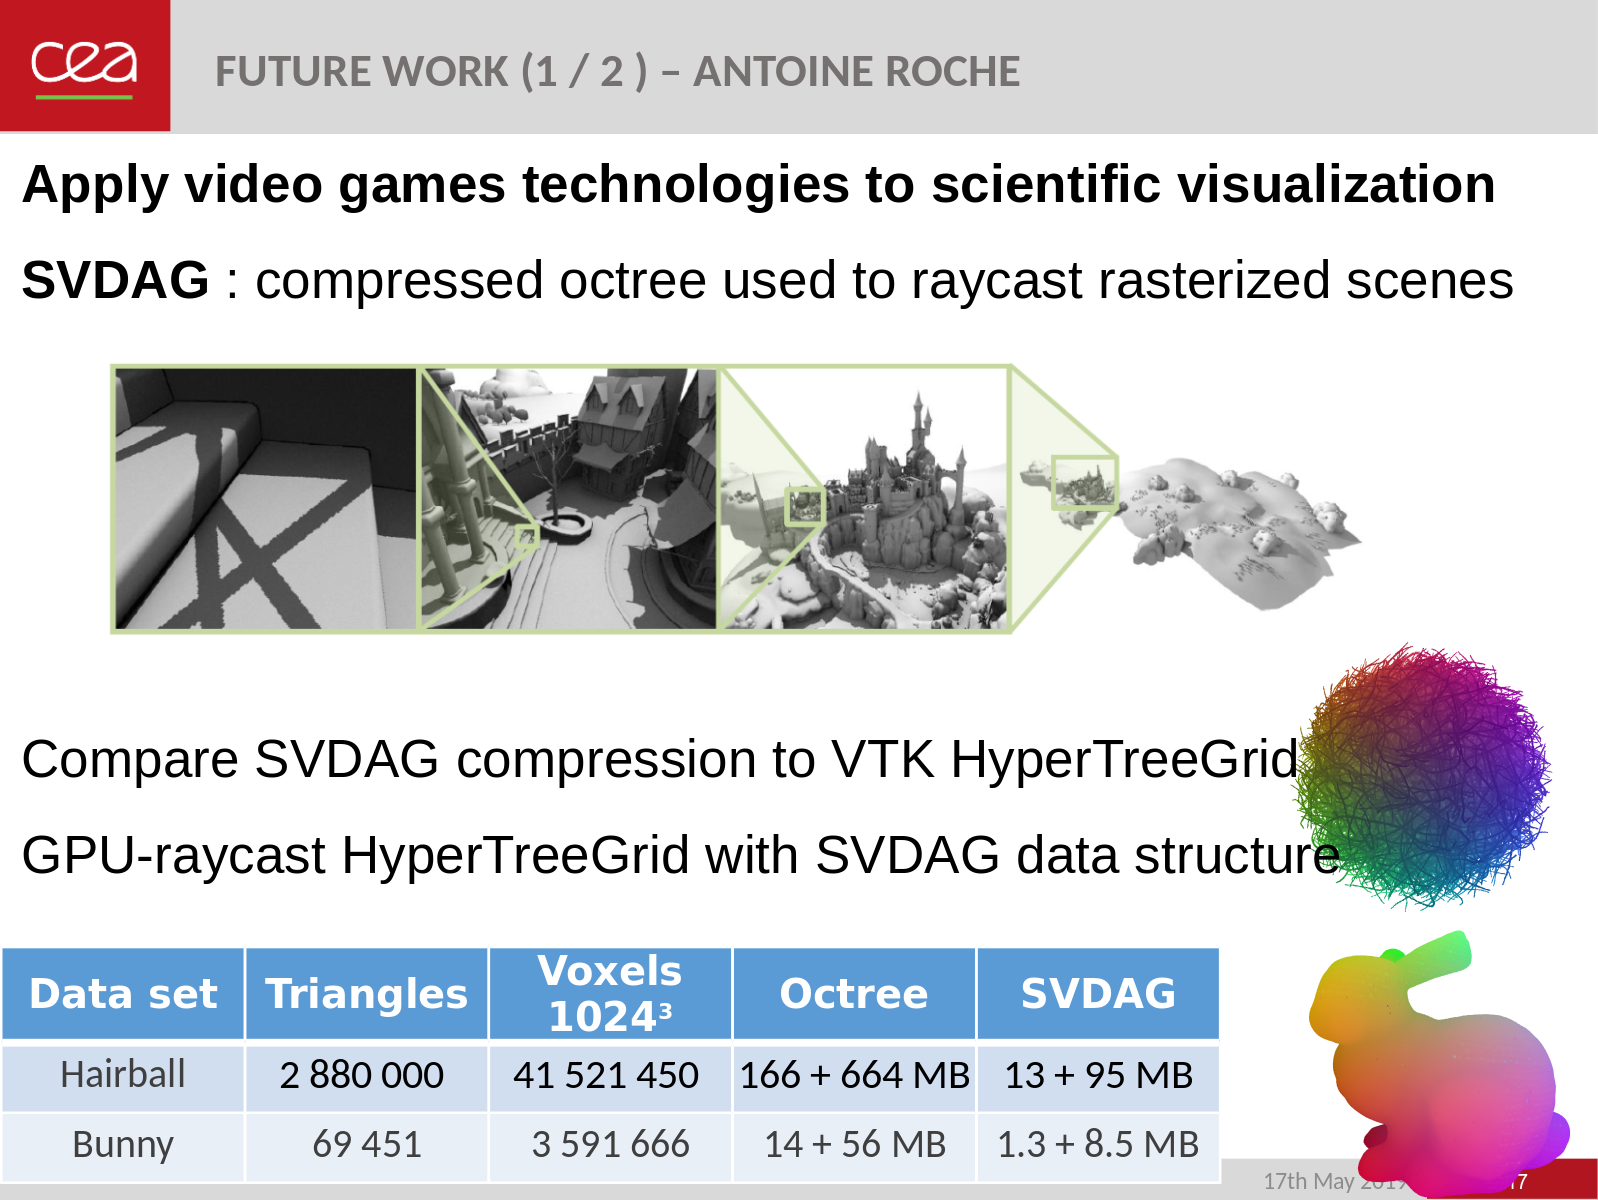
\includegraphics{ressources/images/slide_visu.png}}
        \label{slide_visu}
        }
    \end{figure}

    \section{Expérience personnelle et professionnelle}
    \subsection{Collaboration et contribution}

    \subsubsection{Université de Chamblers}

    Afin de comprendre certaines choses sur le SVDAG, j'ai sollicité Dan Dolonius et Ulf Assarsson, deux chercheurs de l'Université de Chamblers à l'origine du SVDAG.
    La collaboration n'a pas beaucoup abouti, j'ai cependant eu l'occasion des les renseigner sur la compatibilité vers Unix.\\
    De plus, le programme fourni est une ancienne version de ce qu'ils possèdent actuellement, et en avoir une plus récente
    nous permettrait beaucoup plus de choses.

    \subsubsection{CEA}

    Quant à VTK et à l'AMR, Jérôme Dubois et Jacques-Bernard Lekien, contributeurs à VTK, m'ont beaucoup expliqué
    le fonctionnement de la structure AMR et sa construction, me donnant de bonnes bases pour la suite.

    \subsubsection{Journée Visu2019}

    A l'occasion de la journée de la visualisation 2019 se déroulant à Paris le 17 mai, j'ai pu présenter mon travail
    aux personnes présentes en m'appuyant sur la slide produite. Cela a suscité l'intérêt de certains chercheurs,
    demandant par exemple si mon travail pourrait être intégré à VTK.




    \newpage
    \subsection{Problèmes rencontrés}

    \subsubsection{Installations}

    Tout d'abord, l'accès aux machines internes a pris du temps, ce qui a retardé les installations de quelques jours.
    De plus, les restrictions de l'entreprises nous empêchant d'utiliser curl et wget comme bon nous semble, il a donc fallu créer des miroirs.
    Utiliser Roméo pour cela était la meilleure solution. Cependant, une coupure de courant sur le campus survint au mauvais moment.
    La seule façon de faire était de télécharger les paquets un par un via un navigateur et de les placer dans un miroir.

    Concernant VTK, l'installateur télécharge des programmes de test, ce qui bloquait tout. Et les télécharger à la main n'était
    pas envisageable étant donné leur grand nombre. Nous avons donc attendu le retour de Roméo pour les télécharger puis les transférer en ssh.
    \\De plus, l'installation de VTK pour python est en option, ce que je ne savais pas, et les programmes d'exemples qui m'étaient
    donnés étaient en python. Après plusieurs heures de recherches sur l'importation de VTK (car je pensais toujours que VTK python était installé),
    j'ai fini par restranscrire les exemples en C++, ce qui m'a permis au passage de comprendre les différentes étapes.

    \subsubsection{SVDAG}

    Le problème de compatibilité expliqué plus haut m'a également pris beaucoup de temps. En effet, en plus du paquet dépendant au système,
    l'appel d'une fonction template externe ne passait pas à la compilation. Les solutions sur internet liées à l'erreur
    retournée ne parlant que de la fonction en elle-même et non de son appel, j'ai du en partie comprendre les types des
    paramètres donnés (qui étaient des vecteurs très complexes) afin de trouver la source du problème.

    \newpage
    \section{Travaux futurs}

    Durant le reste du stage, mon travail consistera dans un premier temps à prendre connaissance du SSVDAG, pour le
    comparer avec le SVDAG et voir quel est le plus intéressant. Ensuite, je devrai maitriser la structure VTK-AMR en créant un
    AMR à partir d'un SVO en obtenant le même résultat, pour par la suite faire un convertisseur AMR vers SVDAG/SSVDAG.
    Ensuite, des rendus seront faits à partir de données AMR afin d'évaluer les performances et les améliorations possibles.

    \newpage
    \section{Conclusion}                            %%% CONCLUSION %%%

    Manipuler des structures de données complexes demande beaucoup de recherches préliminaires. De plus, certains
    problèmes m'ont fait perdre beaucoup de temps. De ce fait, rien de concret n'a encore été implémenté.\\
    Cependant, les résultats obtenus sont encourageants pour la suite. La familiarisation avec l'environnement de travail
    me permet désormais de travailler plus efficacement qu'au début du stage.

    Le domaine de la recherche en visualisation scientifique est nouveau pour moi, et j'en tire toujours plus
    d'expérience chaque jour, m'encourageant d'avantage à mener ce projet à son terme.

    \newpage
    \section{Glossaire}                             %%% GLOSSAIRE %%%
    Obligatoire dans le rapport


    \newpage
    \section{Bibliographie}                         %%% BIBLIOGRAPHIE %%%

    \bibliographystyle{plain}
    \bibliography{biblio}\nocite{*}


\end{document}